\documentclass[10pt,aspectratio=169]{beamer}

\usetheme[progressbar=foot]{metropolis}
\AtBeginSection{}

\usepackage{appendixnumberbeamer}
\usepackage{booktabs}
\usepackage[scale=2]{ccicons}
\usepackage{tabularx}
\usepackage{tikz}
\usetikzlibrary{arrows.meta,positioning,shapes.geometric}
\usepackage{xspace}
\newcommand{\themename}{\textbf{\textsc{metropolis}}\xspace}
\usepackage{comment}
\usepackage{caption}
\usepackage[
  backend=biber,
  style=authoryear
]{biblatex}

\setbeamertemplate{bibliography item}{}
\addbibresource{bibliography.bib}

\usepackage{graphicx}
\usepackage{siunitx}



%................................................................................
% COLORS

\definecolor{ukudlaBlue}{RGB}{41, 60, 135}
\definecolor{ukudlaLightBlue}{RGB}{212, 216, 231}
\definecolor{ukudlaRed}{RGB}{164, 28, 34}
\definecolor{ukudlaLightRed}{RGB}{236, 209, 210}
\definecolor{ukudlaGreen}{RGB}{59, 139, 71}
\definecolor{ukudlaLightGreen}{RGB}{215, 231, 218}
\definecolor{ukudlaYellow}{RGB}{239, 198, 44}
\definecolor{ukudlaLightYellow}{RGB}{251, 243, 212}
\definecolor{white}{RGB}{255, 255, 255}
\definecolor{black}{RGB}{0, 0, 0}

\setbeamercolor{palette primary}{fg=white, bg=ukudlaGreen}
\setbeamercolor{progress bar}{fg=ukudlaRed, bg=ukudlaYellow}
\setbeamercolor{title separator}{fg=ukudlaRed, bg=ukudlaYellow}
\setbeamercolor{progress bar in head/foot}{fg=ukudlaRed, bg=ukudlaYellow}
\setbeamercolor{progress bar in section page}{fg=ukudlaRed, bg=ukudlaYellow}
\setbeamercolor{background canvas}{bg=white}



%................................................................................
% PRESENTATION INFORMATION

\title{UKUDLA Data Science Certificate}
\subtitle{Version Control and Collaboration using Git \& GitHub}
\author{Markus Mößler}
\institute{University of Hohenheim}



%................................................................................
% CUSTOM FOOTER

\setbeamertemplate{progress bar in head/foot}{%
  \begin{tikzpicture}[overlay, x=\paperwidth, y=1cm]

    % progress bar background
    \fill[ukudlaLightGreen]
      (0,0) rectangle (1,0.10);

    % progress bar foreground
    \fill[ukudlaGreen]
      (0,0) rectangle
      ({\insertframenumber/\inserttotalframenumber},0.10);

    % logo
    \node[
      anchor=south west,
      yshift=0.25cm,
      xshift=0.2cm
    ] at (0,0) {
      \includegraphics[height=0.75cm]
        {./logos/UKUDLA_logo_03_white_bg.pdf}
    };

    % current section
    \ifnum\value{section}>0
      \node[
        anchor=south east,
        yshift=0.22cm,
        xshift=-0.60cm,
        fill=ukudlaLightGreen,
        rounded corners=2pt,
        inner xsep=6pt,
        inner ysep=3pt,
        font=\scriptsize\bfseries,
        text=ukudlaRed
      ] at (1,0) {
        \insertsectionhead
      };
    \fi

  \end{tikzpicture}%
}



%................................................................................
% CUSTOM TITLE PAGE

\makeatletter
\setbeamertemplate{title page}{
  \begin{beamercolorbox}[sep=8pt, center, wd=\paperwidth, ht=0.5\paperheight]{title page top}
    \begin{minipage}[c]{1.00\textwidth}
      \raggedleft
      \includegraphics[height=1.00cm]{./logos/ukudla_universities.pdf}
      \vspace*{0.2cm}
    \end{minipage}
    \begin{beamercolorbox}[wd=0.9\paperwidth, sep=12pt, left]{top box}
      {\usebeamerfont{title}\usebeamercolor[fg]{title}\inserttitle\par}
      \vskip0.1cm
      {\usebeamerfont{subtitle}\usebeamercolor[fg]{subtitle}\insertsubtitle\par}
    \end{beamercolorbox}
  \end{beamercolorbox}
  \begin{beamercolorbox}[sep=8pt, center, wd=\paperwidth, ht=0.5\paperheight]{title page bottom}
    \begin{beamercolorbox}[wd=0.9\paperwidth, sep=12pt, left]{bottom box}
      \hbox{%
        \hspace*{1em}
        \begin{minipage}[c]{0.40\textwidth}
          \vskip1.0cm
          {\usebeamerfont{author}\usebeamercolor[fg]{author}\insertauthor\par}
          \vskip0.1cm
          {\usebeamerfont{institute}\usebeamercolor[fg]{institute}\insertinstitute\par}
        \end{minipage}%
        \hspace*{1.5cm}
        \begin{minipage}[c]{1.00\textwidth}
          \includegraphics[height=2.0cm]{./logos/UKUDLA_logo_05.pdf}
        \end{minipage}%
      }
    \end{beamercolorbox}
    \begin{minipage}[r]{1.00\textwidth}
      \centering
      \includegraphics[width=1.00\textwidth]{./logos/ukudla_sponsors.pdf}
    \end{minipage}
  \end{beamercolorbox}
}
\makeatother

\setbeamercolor{title page top}{bg=white}
\setbeamercolor{top box}{bg=ukudlaGreen}
\setbeamercolor{title page bottom}{bg=white}
\setbeamercolor{bottom box}{bg=ukudlaLightGreen}
\setbeamercolor{title}{fg=white}
\setbeamercolor{subtitle}{fg=white}
\setbeamercolor{author}{fg=black}
\setbeamercolor{institute}{fg=black}
\setbeamercolor{date}{fg=black}

\setbeamercolor{block body}{bg=ukudlaLightGreen,fg=black}



%................................................................................
% DOCUMENT

\begin{document}

\maketitle

%--------------------------------------------------
{
\setbeamertemplate{frame numbering}[none]

\begin{frame}[noframenumbering]{Table of contents}

  \small
  \setbeamertemplate{section in toc}[sections numbered]
  \tableofcontents[hideallsubsections]

\end{frame}
}
%--------------------------------------------------


\section{Motivation}


%--------------------------------------------------
% CONTENT SLIDE 1/10
\begin{frame}[fragile]{Why version a data science project?}

\small

\begin{columns}[T]

\column{0.42\textwidth}

\begin{verbatim}
analysis.R
analysis-new.R
analysis-final.R
analysis-final-revised.R
analysis-final-revised-2.R
\end{verbatim}

\column{0.56\textwidth}

\textbf{Version control provides}

\begin{itemize}
  \item one authoritative project;
  \item a traceable sequence of changes;
  \item meaningful recovery points;
  \item parallel and reviewable work; and
  \item a link between decisions and results.
\end{itemize}

\end{columns}

\vspace{0.25cm}

\begin{beamercolorbox}[rounded=true,sep=8pt]{block body}
Saving a file is not the same as recording a version. Version control turns a
folder of files into a project with a documented history.
\end{beamercolorbox}

\end{frame}
%--------------------------------------------------


%--------------------------------------------------
% CONTENT SLIDE 2/10
\begin{frame}{Why this matters for food-systems data science}

\small

Food-systems analyses combine many changing elements:

\begin{itemize}
  \item data-acquisition and cleaning decisions;
  \item definitions, units, study units, and time periods;
  \item statistical code and model specifications;
  \item figures, reports, and interpretation; and
  \item software-environment descriptions.
\end{itemize}

\vspace{0.25cm}

\begin{beamercolorbox}[rounded=true,sep=9pt]{block body}
A small change in a filtering rule or unit conversion can change the scientific
conclusion.

\vspace{0.1cm}

Git helps connect that conclusion to a specific, inspectable state of the
project.
\end{beamercolorbox}

\end{frame}
%--------------------------------------------------


\section{Concepts}


%--------------------------------------------------
% CONTENT SLIDE 3/10
\begin{frame}{Git and GitHub: local history and shared collaboration}

\small

\begin{columns}[T]

\column{0.46\textwidth}

\textbf{Git}

\begin{itemize}
  \item Distributed version control system
  \item Runs on the local computer
  \item Records project snapshots
  \item Most operations work offline
\end{itemize}

\column{0.48\textwidth}

\textbf{GitHub}

\begin{itemize}
  \item Online platform hosting Git repositories
  \item Provides a shared remote location
  \item Adds review and access control
  \item Supports issues, pull requests, and automation
\end{itemize}

\end{columns}

\vspace{0.50cm}

\centering

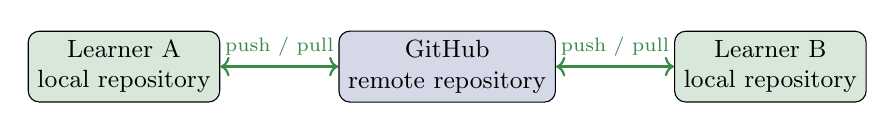
\begin{tikzpicture}[
  box/.style={
    draw,
    rounded corners,
    minimum height=0.80cm,
    minimum width=2.35cm,
    align=center,
    fill=ukudlaLightGreen,
    font=\small
  },
  remote/.style={box,fill=ukudlaLightBlue},
  arrow/.style={-{Latex[length=2mm]},thick,ukudlaGreen}
]
  \node[box] (a) {Learner A\\local repository};
  \node[remote, right=1.5cm of a] (gh) {GitHub\\remote repository};
  \node[box, right=1.5cm of gh] (b) {Learner B\\local repository};
  \draw[arrow,<->] (a) -- node[above,font=\scriptsize]{push / pull} (gh);
  \draw[arrow,<->] (gh) -- node[above,font=\scriptsize]{push / pull} (b);
\end{tikzpicture}

\end{frame}
%--------------------------------------------------


%--------------------------------------------------
% CONTENT SLIDE 4/10
\begin{frame}{A commit is a meaningful project snapshot}

\small

A commit records selected changes with an author, timestamp, message, and
connection to the preceding project history.

\vspace{0.25cm}

\centering

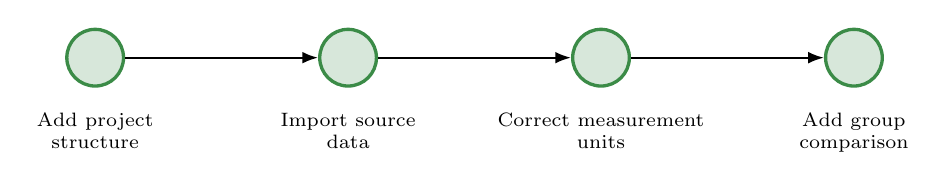
\begin{tikzpicture}[
  commit/.style={
    circle,
    draw=ukudlaGreen,
    very thick,
    fill=ukudlaLightGreen,
    minimum size=0.72cm
  },
  label/.style={align=center,font=\scriptsize},
  arrow/.style={-{Latex[length=2mm]},thick}
]
  \node[commit] (c1) {};
  \node[commit, right=2.45cm of c1] (c2) {};
  \node[commit, right=2.45cm of c2] (c3) {};
  \node[commit, right=2.45cm of c3] (c4) {};
  \draw[arrow] (c1) -- (c2);
  \draw[arrow] (c2) -- (c3);
  \draw[arrow] (c3) -- (c4);
  \node[label, below=0.20cm of c1] {Add project\\structure};
  \node[label, below=0.20cm of c2] {Import source\\data};
  \node[label, below=0.20cm of c3] {Correct measurement\\units};
  \node[label, below=0.20cm of c4] {Add group\\comparison};
\end{tikzpicture}

\vspace{0.25cm}

\raggedright

\begin{itemize}
  \item A commit should contain one coherent change.
  \item The diff records \emph{what} changed.
  \item The message should help explain \emph{why}.
\end{itemize}

\end{frame}
%--------------------------------------------------


%--------------------------------------------------
% CONTENT SLIDE 5/10
\begin{frame}{From an edited file to shared history}

\centering

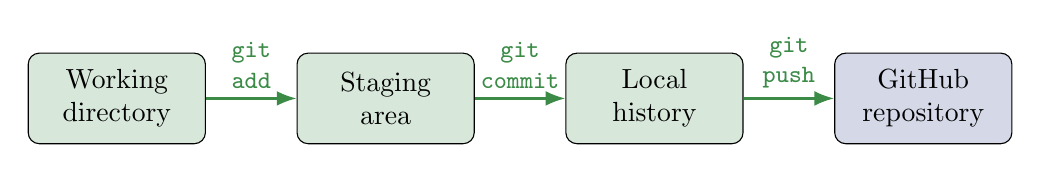
\begin{tikzpicture}[
  state/.style={
    draw,
    rounded corners,
    minimum height=1.15cm,
    minimum width=2.25cm,
    align=center,
    fill=ukudlaLightGreen
  },
  remote/.style={state,fill=ukudlaLightBlue},
  arrow/.style={-{Latex[length=2.5mm]},thick,ukudlaGreen},
  command/.style={font=\small\ttfamily}
]
  \node[state] (work) {Working\\directory};
  \node[state, right=1.15cm of work] (stage) {Staging\\area};
  \node[state, right=1.15cm of stage] (history) {Local\\history};
  \node[remote, right=1.15cm of history] (remote) {GitHub\\repository};

  \draw[arrow] (work) --
    node[above,command,align=center]{git\\add} (stage);
  \draw[arrow] (stage) --
    node[above,command,align=center]{git\\commit} (history);
  \draw[arrow] (history) --
    node[above,command,align=center]{git\\push} (remote);
\end{tikzpicture}

\vspace{0.50cm}

\small

\begin{columns}[T]

\column{0.49\textwidth}

\textbf{Workflow}

\begin{itemize}
  \item Editing changes the working directory.
  \item Staging selects what belongs to the next commit.
  \item Committing records a local snapshot.
  \item Pushing shares local commits with the remote repository.
\end{itemize}

\column{0.49\textwidth}

\textbf{Not everything should be tracked!}

\begin{itemize}
  \item secrets and credentials;
  \item confidential data;
  \item large downloaded data;
  \item generated outputs;
  \item package libraries and caches; and
  \item editor-specific state.
\end{itemize}

\end{columns}

\end{frame}
%--------------------------------------------------


%--------------------------------------------------
% CONTENT SLIDE 6/10
\begin{comment}
\begin{frame}[fragile]{Inspect, select, record and share}

\small

\begin{columns}[T]

\column{0.52\textwidth}

\begin{verbatim}
git status
git diff
git add path/to/file
git diff --staged
git commit -m "Correct measurement units"
git push
\end{verbatim}

\column{0.46\textwidth}

\textbf{Before committing}

\begin{itemize}
  \item Do I understand each change?
  \item Do these changes belong together?
  \item Did I include private or generated files?
  \item Does the project still work?
\end{itemize}

\end{columns}

\vspace{0.20cm}

\begin{beamercolorbox}[rounded=true,sep=8pt]{block body}
\texttt{Correct measurement unit conversion} communicates a decision.
\texttt{changes}, \texttt{stuff}, and \texttt{final} do not.
\end{beamercolorbox}

\end{frame}
%--------------------------------------------------
\end{comment}
%--------------------------------------------------
\begin{frame}[fragile]{Inspect before you record}

\small

\begin{verbatim}
git status
git diff
git add path/to/file
git diff --staged
git commit -m "Correct measurement unit conversion"
git push
\end{verbatim}

\vspace{0.25cm}

\begin{columns}[T]

\column{0.49\textwidth}
\textbf{Questions before committing}

\begin{itemize}
  \item Do I understand each change?
  \item Do these changes belong together?
  \item Did I include generated or private files?
\end{itemize}

\column{0.49\textwidth}
\textbf{A useful commit}

\begin{itemize}
  \item is small and coherent;
  \item leaves the project usable; and
  \item explains why the change matters.
\end{itemize}

\end{columns}

\end{frame}
%--------------------------------------------------


\section{Application}


%--------------------------------------------------
% CONTENT SLIDE 7/10
\begin{frame}{A collaborative Git cycle}

\small

\centering
\Large
\texttt{inspect} $\rightarrow$ \texttt{pull} $\rightarrow$ \texttt{edit}
$\rightarrow$ \texttt{commit} $\rightarrow$ \texttt{push}

\vspace{0.25cm}

\normalsize
\raggedright

\begin{itemize}
  \item Pull remote changes before beginning a new task.
  \item Make small, focused changes.
  \item Communicate which files or tasks people are working on.
  \item Push completed commits so collaborators can build on them.
  \item Integrate frequently; long-lived divergence increases effort.
\end{itemize}

\vspace{0.25cm}

\begin{beamercolorbox}[rounded=true,sep=8pt]{block body}
Collaboration means exchanging and integrating commits---not emailing copies of
``final'' files.
\end{beamercolorbox}

\end{frame}
%--------------------------------------------------


%--------------------------------------------------
% CONTENT SLIDE 8/10
\begin{frame}{Divergence, merging and scientific judgment}

\small

\begin{columns}[T]

\column{0.44\textwidth}

\centering

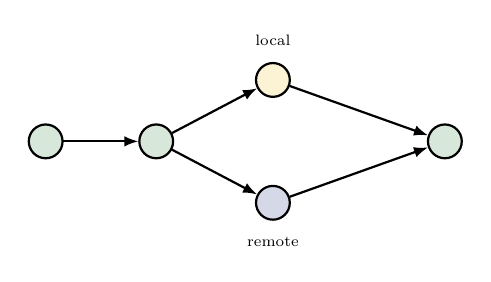
\begin{tikzpicture}[
  commit/.style={
    circle,
    draw,
    thick,
    fill=ukudlaLightGreen,
    minimum size=0.55cm
  },
  local/.style={commit,fill=ukudlaLightYellow},
  remote/.style={commit,fill=ukudlaLightBlue},
  arrow/.style={-{Latex[length=1.8mm]},thick},
  scale=0.78,
  transform shape
]
  \node[commit] (base) at (0,0) {};
  \node[commit] (shared) at (1.8,0) {};
  \node[local] (local) at (3.7,1.0) {};
  \node[remote] (remote) at (3.7,-1.0) {};
  \node[commit] (merged) at (6.5,0) {};
  \draw[arrow] (base) -- (shared);
  \draw[arrow] (shared) -- (local);
  \draw[arrow] (shared) -- (remote);
  \draw[arrow] (local) -- (merged);
  \draw[arrow] (remote) -- (merged);
  \node[above=0.15cm of local,font=\scriptsize] {local};
  \node[below=0.15cm of remote,font=\scriptsize] {remote};
\end{tikzpicture}

\column{0.54\textwidth}

\begin{itemize}
  \item Diverging histories are normal.
  \item Git often combines different changes automatically.
  \item A conflict asks a human to choose or integrate.
  \item The integrated analysis must still run and retain its intended meaning.
\end{itemize}

\end{columns}

\vspace{0.30cm}

\begin{beamercolorbox}[rounded=true,sep=8pt]{block body}
Git identifies overlapping text. It cannot decide which research assumption,
data transformation, or interpretation is scientifically correct.
\end{beamercolorbox}

\end{frame}
%--------------------------------------------------


%--------------------------------------------------
% CONTENT SLIDE 9/10
\begin{frame}{Version control supports the complete data science workflow}

\centering

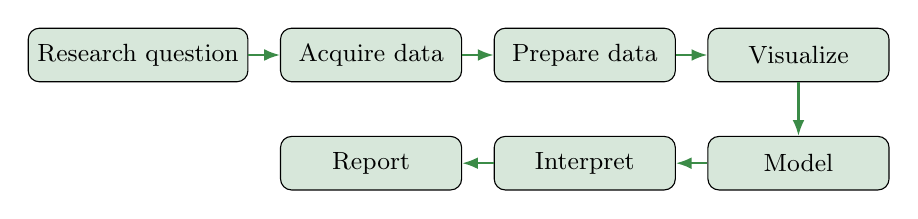
\begin{tikzpicture}[
  workflowstep/.style={
    draw,
    rounded corners,
    minimum height=0.68cm,
    minimum width=2.30cm,
    align=center,
    font=\small,
    fill=ukudlaLightGreen
  },
  arrow/.style={-{Latex[length=2mm]},thick,ukudlaGreen}
]
  \node[workflowstep] (q) {Research question};
  \node[workflowstep, right=0.40cm of q] (acq) {Acquire data};
  \node[workflowstep, right=0.40cm of acq] (prep) {Prepare data};
  \node[workflowstep, right=0.40cm of prep] (viz) {Visualize};
  \node[workflowstep, below=0.68cm of viz] (model) {Model};
  \node[workflowstep, left=0.40cm of model] (interpret) {Interpret};
  \node[workflowstep, left=0.40cm of interpret] (report) {Report};

  \draw[arrow] (q) -- (acq);
  \draw[arrow] (acq) -- (prep);
  \draw[arrow] (prep) -- (viz);
  \draw[arrow] (viz) -- (model);
  \draw[arrow] (model) -- (interpret);
  \draw[arrow] (interpret) -- (report);
\end{tikzpicture}

\vspace{0.25cm}

\small

\begin{columns}[T]

\column{0.49\textwidth}

\textbf{Git and GitHub}

\begin{itemize}
  \item mark meaningful stages;
  \item connect code changes to results; and
  \item support sharing and review.
\end{itemize}

\column{0.49\textwidth}

\textbf{Track deliberately}

\begin{itemize}
  \item Track code, documentation, and lockfiles.
  \item Exclude secrets, sensitive data, caches, and unsuitable large files.
\end{itemize}

\end{columns}

\end{frame}
%--------------------------------------------------


\section{Key Message}


%--------------------------------------------------
% CONTENT SLIDE 10/10
\begin{frame}{Key message: version meaningful project states}

\large

\begin{enumerate}
  \item Git records meaningful states of a project.
  \item GitHub provides a shared location and collaboration tools.
  \item Inspecting changes is part of responsible data science.
  \item Small commits and frequent synchronization reduce problems.
  \item Version control supports reproducibility, but does not replace data, environment, and workflow documentation.
\end{enumerate}

\vspace{0.25cm}

\small
\centering

Detailed setup, repository, workflow, and troubleshooting instructions are provided in the learning-module guides.

\end{frame}
%--------------------------------------------------


%--------------------------------------------------
\begin{frame}[plain,noframenumbering]{Supported by}

  South African government and the National Research Foundation

  \begin{flushleft}
    \includegraphics[trim=0cm 0cm 0cm 0cm, clip, width=0.50\textwidth]{./logos/ukudla_south_african_sponsors.pdf}
  \end{flushleft}

  German government and the German Academic Exchange Service

  \begin{flushleft}
    \includegraphics[trim=0cm 0cm 0cm 0cm, clip, width=1.00\textwidth]{./logos/ukudla_german_sponsors.pdf}
  \end{flushleft}

\end{frame}
%--------------------------------------------------

\end{document}
